\cleartooddpage[\thispagestyle{empty}]
\chapter{Gamma Ray Reconstruction Methods}\label{ch:grrecon}

In Chapter \ref{chapter:veritas}, it was explained how the trigger system initializes the readout of PMT voltage traces.
To reconstruct gamma rays, the voltage traces induced by Cherenkov photons must be identified and combined to form an image of the original Cherenkov shower.
Then the shower images from multiple telescopes can be used to reconstruct the original gamma ray's energy and direction.

\section{Pedestal Variation}
  Before reconstructing any events, the pedestal and pedestal variations must be calculated.
  This is done by artificially triggering all pixels once per second during observations, in order to record events that contain only noise.
  The average of the digital counts (dc) of all noise events for each pixel is then the pedestal.
  From this pedestal, the pedestal variations are then calculated for each pixel as the rms of all the dc counts in all noise events, which can be visualized as the distribution of dc around the mean dc.
  In this context, noise events can be due to night-sky-background photons, or from electronic noise.

\section{Pixel Identification}
  The first step is to determine which pixels are part of a shower image.
  This is done by subtracting the dc pedestal from the entire trace, and then summing all trace bins within a fixed window, called the integration length, to get the total dc.

  Most voltage traces have the same general shape: a quickly rising start of the pulse, followed by a longer, slowly falling tail.
  To act as a point of reference in each voltage pulse, the time when the voltage trace is at half of its maximum value is called $T_{0}$.
  The trace is then integrated a second time using a smaller 14 or \SI{24}{ns}-wide time window, starting at $T_0 - 30\%$, to reduce the inclusion of dc from NSB photons and electronic noise.
  This integration is the first of two passes, usually referred to as the double-pass method \cite{doublepass}.
  If a pixel's first-pass total dc is higher than 5 times the pedestal variation, then it is classified as an image pixel.
  If it is between 2.5 and 5 times the pedestal variation, it is considered a border pixel.

  Once all pixels have been classified, isolated border pixels that have no neighboring image pixel are removed from the image, as they are more likely to be due to noise than Cherenkov photons.
  Then, the time gradient from the image and border pixels can be found by performing a linear fit of the $T_{0}$ times.
  This time gradient can then be used to place a third integration window for a 
with 30\% of the window before each pixel's $T_{0}$, to more accurately measure the charge due to Cherenkov photons in the pixel.
  This third integration window is the second pass in the double-pass method.

  From the image pixels, border pixels, and time gradient, the shower's Hillas parameters \cite{hillas_params} can be calculated.
  These parameters include the shower size in photoelectrons (or equivalent units), center of charge, angle, length, and width.
  The center of charge is the charge-weighted average of all image and border pixel positions.
  The angle of the shower determines how the image's major axis is oriented in the camera.
  The shower length and width are determined by the rms of the shower image along its major and minor axes, respectively.

\section{Position Reconstruction}\label{subsec:posrecon}
  By examining the images from multiple telescopes, the initial position of the event can be determined.
  This is done by overlapping all telescope images in a single camera coordinate system, and projecting each image's major axis backward in time.
  These axes should intersect very close together, and the average of the intersection points determines the event's initial direction.

  In averaging the intersection points, weighting for each intersection can be applied based on the angle between the two lines.
  This improves the reconstruction, because the intersection point from two images at \ang{90} angles will be less sensitive to image fluctuations than two images at \ang{160}, as shown in Figure \ref{fig:largeintersectangle}.
  Additionally, the disp method described in Section \ref{subsec:disp} can be utilized to offer improvements at lower telescope elevations.

  \begin{figure}[ht]
    \centering
    \includegraphics[width=0.95\textwidth]{images/large_angle_image_intersection_error/laiie_cropped.pdf}
    \caption[Large Image Intersection Angles]{
      In diagram (a), when a noisy pixel is added to an image, the reconstructed position is only moved a small distance (the purple arrow).
      In diagram (b), due to the large angle between images, the error in the reconstructed position is much larger.
    }
    \label{fig:largeintersectangle}
  \end{figure}
  \FloatBarrier

  \subsection{Angular Reconstruction with Boosted Decision Trees}\label{subsec:disp}
    At high elevations, shower images often form small intesection angles, because the telescopes are spread out in two dimensions, relative to the shower in the atmosphere.
    At low elevations near the Galactic Center, however, the telescope array flattens into one dimension, which makes the shower's impact parameter (the shortest distance between the telescope and the shower core axis) smaller for two of the telescopes.
    These two closer telescopes then have very short, almost circular images, which increases the sensitivity of those two image axes to noisy pixels or shower fluctuations, as shown in Figure \ref{fig:showerhighlowelev}.
    This also causes the remaining telescope images to have large intersection angles, which also reduces the accuracy of the position reconstruction.

    \begin{figure}[ht]
      \centering
      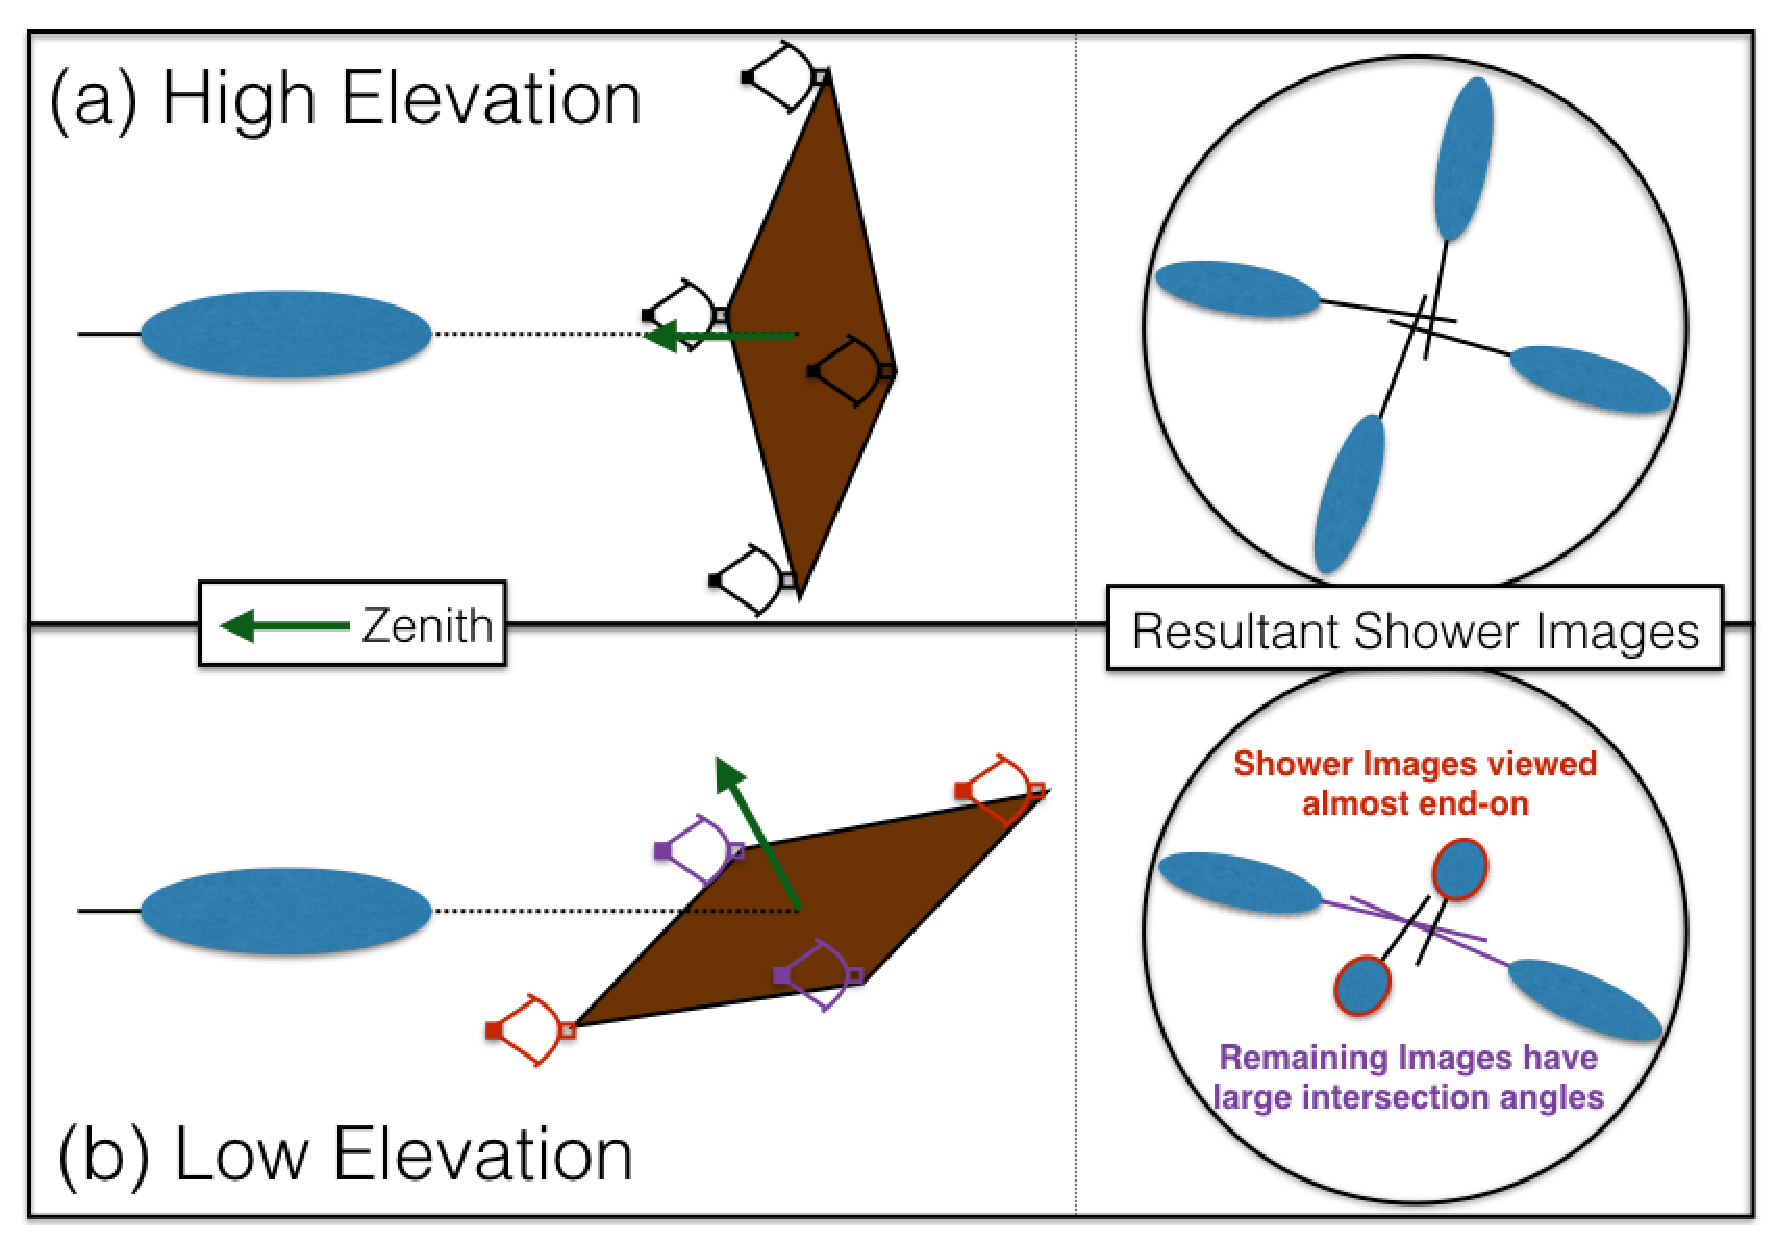
\includegraphics[width=0.75\textwidth]{images/high_elevation_vs_low_shower_images_cropped.eps}
      \caption[Shower Images at High and Low Elevations]{
        In Figure (a), high elevation showers produce long images in all four telescopes.
        In Figure (b), lower elevation showers produce shortened images in two telescopes, and the remaining images form large angle intersection.
      }
      \label{fig:showerhighlowelev}
    \end{figure}

    To better handle these near-parallel image axes at low elevations, the reconstructed position can be determined from more parameters than just the weighted intersection points from the image axes.
    From simulations, the distance between the center of the Hillas shower image and the true position can be calculated, where the angular distance between the two is the \disp{} parameter~\cite{Senturk:2011}, shown in Figure \ref{fig:dispdiagram}.
    Then, this \disp{} parameter can be provided to a machine learning algorithm \cite{Beilicke2012NIM}, along with other image parameters like:
    \begin{description}
      \item[\textit{width}:] image angular width
      \item[\textit{length}:] image angular length
      \item[\textit{wol}:] $\frac{\textrm{width}}{\textrm{length}}$
      \item[\textit{size}:] total image dc
      \item[\textit{ntubes}:] number of pixels in the image
      \item[\textit{loss}:] fraction of image pixels at the edge of the camera
      \item[\textit{asym}:] distance between image center-of-dc and the pixel with the highest dc
      \item[\textit{tgrad}:] the slope of the linear time fit to the pixel arrival times
      \item[\textit{cross}:] angular distance between the image center and the average intersection point of the image axes.
    \end{description}
  % list of training parameters: grep "AddVariable" $EVNDISPSYS/src/trainTMVAforAngularReconstruction.cpp
  % how variables are calculated: grep -P "fParGeo.+\=" $EVNDISPSYS/src/VImageParameterCalculation.cpp
  % asym: http://inspirehep.net/record/1395717/files/RdelosReyes.pdf
  % Once trained on these parameters, the machine learning algorithm can construct a boosted decision tree for determining any new image's \textit{disp}, which can then be used with the image axes intersections to improve the gamma-ray reconstructed positions.


    \begin{figure}[ht]
      \centering
      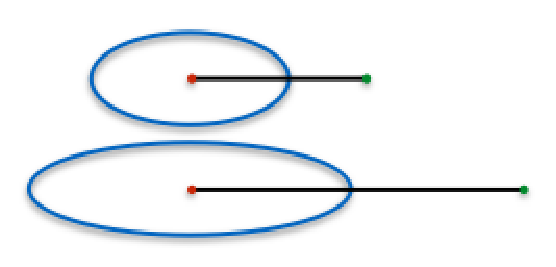
\includegraphics[width=0.5\textwidth]{images/disp_parameter_cropped.eps}
      \caption[Angular Reconstruction Disp]{
        The \disp{} parameter is the angular distance between the center (red dot) of a Hillas image (blue oval) and the true sky position (green dot).
        Generally, longer shower images have a larger \disp{} angle.
      }
      \label{fig:dispdiagram}
    \end{figure}

    % https://veritas.sao.arizona.edu/wiki/index.php/BDT_Angular_reconstruction
    These parameters for thousands of simulated showers can then be used to train boosted decision trees (BDTs) that estimate the \disp{} for a new shower's images.
    This estimated \disp{} can then be used with the image axes intersection points to more accurately reconstruct the original gamma-ray point of origin.
    
    Once the training is complete, it is tested on a separate set of 17,000 simulated events, which have their true and predicted \disp{}s plotted in Figure \ref{fig:disptraining}.
    The x axis describes the true \disp{} value for each event, while the y axis describes the \disp{} value estimated by the BDT, with a black $x=y$ line marked, which represents a perfect 1:1 \disp{} reconstruction.
    As events fall on the $x=y$ line, it can be concluded that the BDTs are able to predict the correct \disp{} value for most images.
    {\color{red} You need to be more precise.  You should show also a one dimenional distribution (or various if you want to divide to True DISP bins) and discuss the resolution obtained?? -Orel}

    % made from screenshot of last slide in Dropbox/Presentations/20160719_Group_Meeting.key
    \begin{figure}[ht]
      \centering
      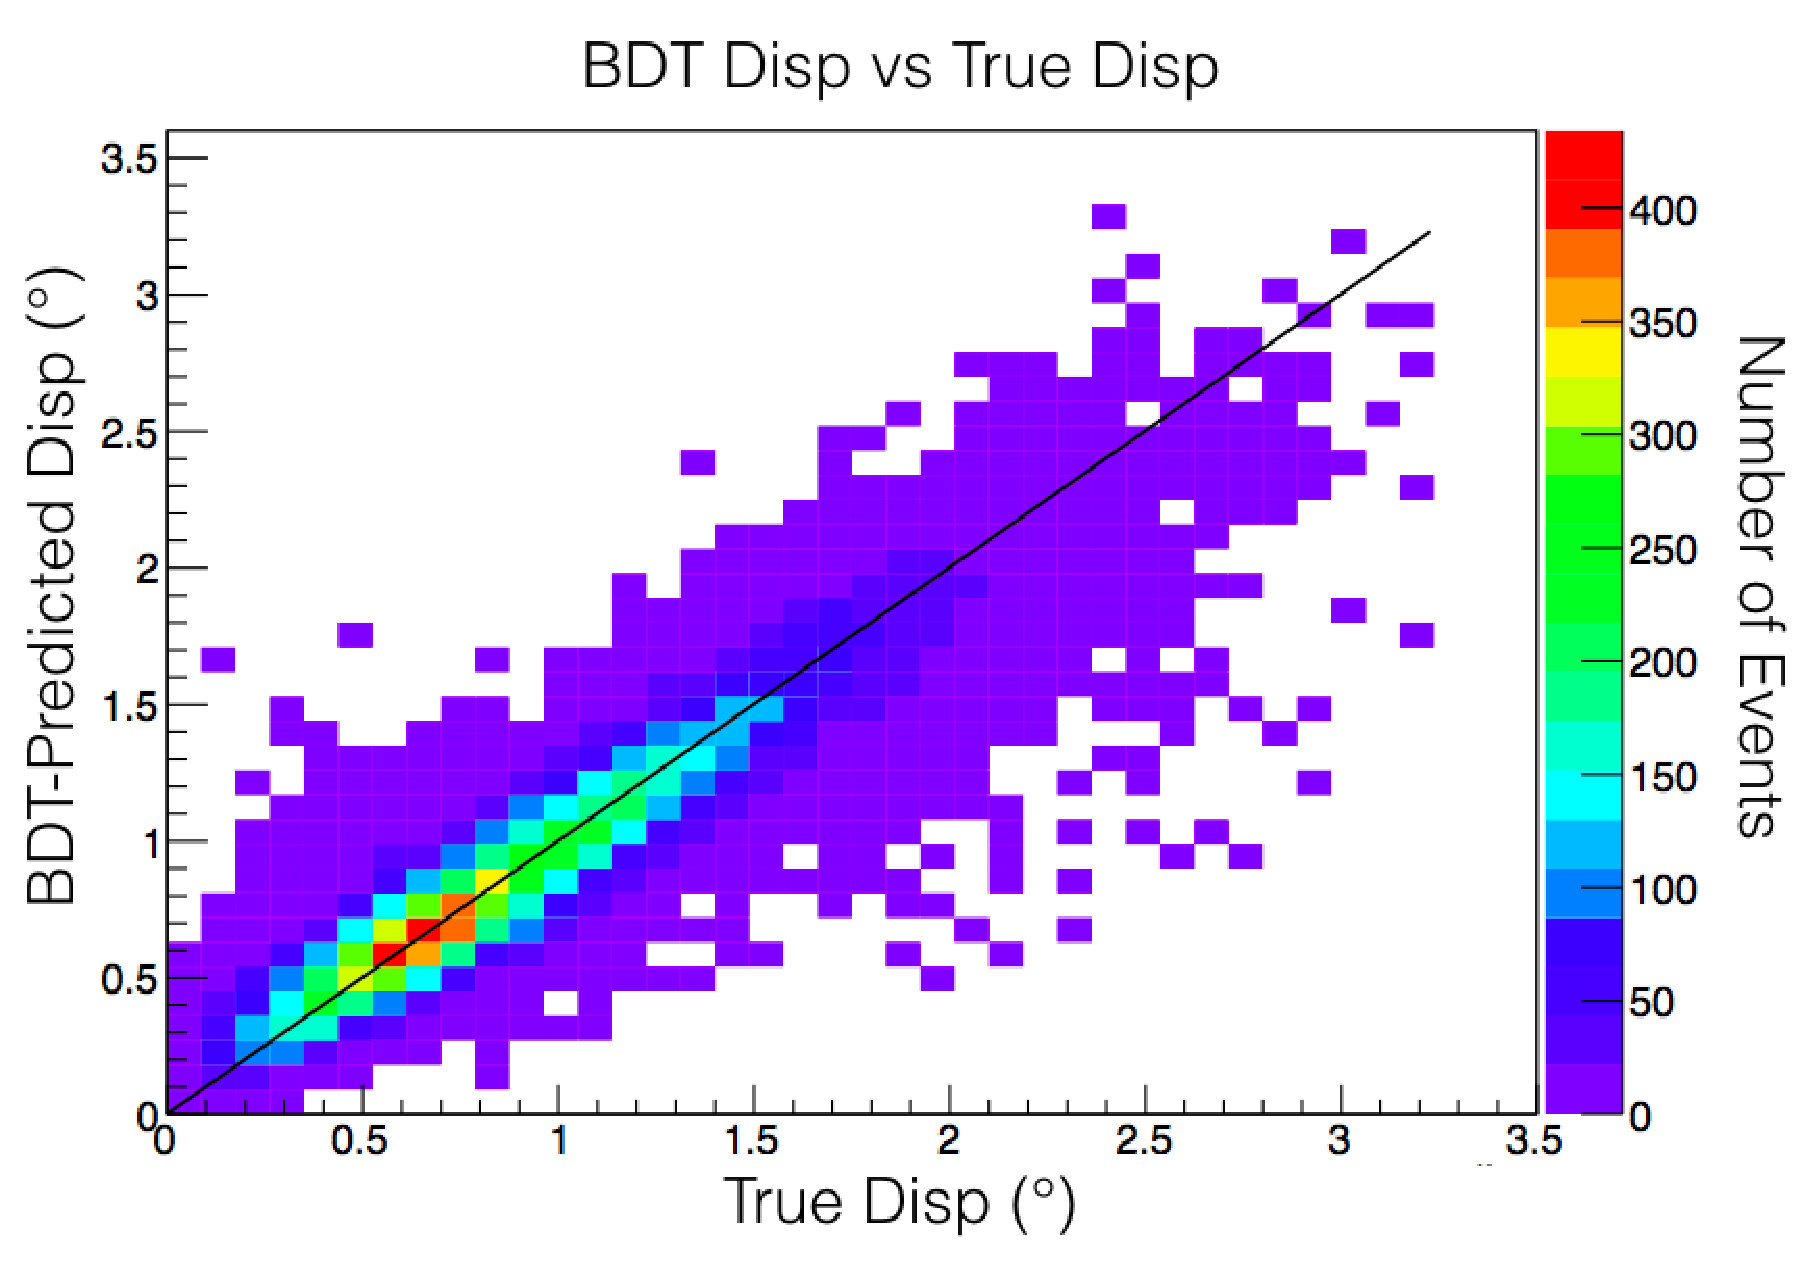
\includegraphics[width=0.85\textwidth]{images/disp_training.eps}
      \caption[Disp BDT Training]{
        The true \disp{} vs the BDT-predicted \disp{}, for \nicetilde17,000 gamma-ray event images in T1, from \SI{500}{\GeV} to \SI{200}{\TeV}.
      }
      \label{fig:disptraining}
    \end{figure}
    
    {\color{red} profile plot of the true/BDT disp vs true disp, with 68\% containment errorbars, and talk about it in the text! is there a bias? at what disps? }

    The small improvement in the position reconstruction due to the \disp{} method can be seen in Figure \ref{fig:disp_event_offset}.
    With the Geometric (red) events, more are concentrated further from the point source, while with the {\color{red}Disp (capitolization??)} method, a few more are concentrated at the source itself.
    
    {\color{red}Again, you need to be more specific. First, it is important to note this is data, it's always good to ''brag`` that your reconstruction method is tested on data.  Second, you need to discuss the actual resolution obtained with both methods and state the improvement achieved with DISP. I think the RMS might be a better test of this and anyway the mean would be too affected by the tail. In fact I think the quantiles are better?? -Orel}
    
    {\color{red} Mention that from here on in the analysis, the disp method is used! ??}
  
    {\color{red}I don't understand why the improvements are so small.  Different ot what I see. -Gernot?? }

    \begin{figure}[ht]
      \centering
      \includegraphics[width=0.85\textwidth]{images/disp_event_offset_hists/dispgeom_comparison.eps}
      \caption[DISP Offset Improvement]{
        The fraction of events at different angular offsets from the Crab and the Galactic Center per solid angle, with Geometric (intersection only) and Disp reconstruction methods.
        Data elevations are the same as in Figure \ref{fig:datapointingelevations}, while training events were simulated at only \ang{28}.
        {\color{red}(Where is the disp improvement???)}
        {\color{red}(Why is the containment radius worse for disp??)}
        {\color{red}(Redo disp training with 5x events! ??)}
        {\color{red}(change y axis label to Disp/Geometric! ??)}
        {\color{red}(Rerun this histogram for different energies, better to say this had some improvements at some energies or offsets than on average it had no effect.}
      }
      \label{fig:disp_event_offset}
    \end{figure}
  
  {\color{red}Also include dispgeom\_comparison\_psftable.crab.png in \$V/thesis/plots , but only focus on my energy range, and switch it to be distributions at each energy}

  \FloatBarrier

\section{Energy Reconstruction}\label{subsec:enrecon}
  To reconstruct the energy of each shower, a lookup table of simulated showers is built.
This database includes the width and length of the shower, how far away its core position is, how bright it was, as well as its reconstructed and true energy.
  By scanning through this database for showers that are similar to the one being constructed, the most similar-looking shower then indicates the true energy {\color{red} (is there any interpolation?? -Orel?? ask gernot)}.


\section{FITS Conversion for Gammalib and CTOOLs}\label{fitsconversion}
  Once gamma rays have been reconstructed with Eventdisplay, they must be converted to a FITS file format compatible with Gammalib and CTOOLS.
  This format consists of a FITS file with an event list table, containing each gamma ray, its energy, sky direction, and time.
  This also includes meta information about the event list like the telescope's pointing target and the start and end times of the event list.
  This FITS file can then be read into Gammalib and CTOOLS \cite{gammalibctools}.

  In addition to the event list, the instrument response functions (IRFs) must also be imported into Gammalib and CTOOLS.
  These IRFs consist of the effective areas, the point spread functions, the background models, and the energy dispersion.
  The effective area quantifies the total gamma-ray collection area of the observatory, needed for spectral measurements, and is described in Section \ref{subsec:effarea}.
  The point spread function (PSF) quantifies the distribution of reconstructed positions for a given true position, which is needed for modeling point sources and extended spatial structures.
  This is described further in Section \ref{subsec:psf}.
  The background models measure the relative number of observed events in different parts of the camera, and their construction is described in Section \ref{background_production}.
  The energy dispersion quantifies the distribution of reconstructed energies for a given true energy, and is discussed in Section \ref{subsec:edisp}.

  Each of these IRFs vary in a parameter space with several dimensions, including event energy, reconstructed distance from the camera center, telescope elevation and azimuth, and night sky background noise.
  In CTOOLS' default configuration, all IRFs are stored in a single directory of files, and each event list contains a filepath reference to indicate which volume of the parameter space it uses.
  Once each volume is loaded, individual events can then interpolate their specific effective area, PSF, and energy dispersion (the backgrounds are utilized differently, as discussed in Section \ref{background_production}).
  {\color{red}All of this information from 5.5 to 5.5.1 on data format and dividing runs to smaller chunks etc. has to be rewritten from the physical point of view and all of the computational references should be removed. I know it sounds weird, but the computational details are of no interest. What's important is the fact you divided your data into smaller bins in order to avoid large changes within each bin.  We can discuss this of course. -Orel??}

  {\color{red}(This paragraph just kind of starts here, theres no transition from the previous paragraph!??)}
  However, the Galactic Center is at an elevation of \ang{30}, much lower than most VERITAS observation targets.
  At this elevation, with its field of view of \ang{3.5}, the airmass column density ($g/cm^{2}$) is 20\% higher at the bottom of the camera than at the top.
  Add to this that during a single 30 minute observation, the elevation of the Galactic Center can change by several degrees.
  This means the airmass in view of the camera may change rapidly, resulting in IRFs that are time dependent.

  To allow for the inclusion of this time dependence in the analysis, observing runs were broken up into smaller time {\color{red}chunks (try to find another word, chunks doesn't work well!??)}, and each time chunk had IRFs assigned to each chunk based on that chunk's position in the elevation/azimuth/night-sky-background-noise parameter space.
  There were minor issues with converting the IRFs, which are noted in the following sections.

  \FloatBarrier
  
  \subsection{Effective Area}\label{subsec:effarea}
    % use effective area as a casual noun!
    % plot of effective area vs energy
    Effective area is the measure of how large an observatory's collection area is, which determines how many gamma rays can be detected per unit time, solid angle, and energy.

    For each point in the parameter space, the effective areas are calculated with many {\color{red}(how many?? -Gernot (probably # corsika showers * number of core rescatters * # camera repositions))} Monte Carlo gamma ray simulations.
    This is done in the shower plane, {\color{red} the plane perpendicular to the line drawn between an observing source, and the center (shower plane depends only on the pointing direction, not on what source is observed -Gernot??)}of the observatory.
    The effective area is then calculated via:
    $A=\pi R^2 \frac{N_{\text{survived}}}{N_{\text{simulated}}}$
    where R is the radius of the area within which simulated showers are directed to fall, $N_{\text{simulated}}$ is the number of showers that were initially simulated into the area, and $N_{\text{survived}}$ is the number of simulated showers that pass all cuts.
    This effective area is thus a measure of how much detection area the observatory would have if it had a 100\% detection efficiency, which can then be used in calculating a source's flux.
    In Figure \ref{fig:effarea_paramspace} shows how the effective area peaks to \nicetilde{}\SI{3e5}{m${}^2$} for \SI{3}{\TeV} events at the camera center.

    \begin{figure}[ht]
      \centering
      \includegraphics[width=0.85\textwidth]{images/effarea_plots/effarea_space.eps}
      \caption[Effective Area Parameter Space]{
        Effective areas at different points in the Energy and Camera Offset parameter space for run 78128.
        Data is shown as the black points, indicating the position of some events from that run in the parameter space.
        The color axis indicates the Effective Area, calculated from simulations, at different gamma-ray energies and distances from the camera center.
        {\color{red}Switch x-axis units to TeV, not log10(TeV)??}
      }
      \label{fig:effarea_paramspace}
    \end{figure}

    For the test analyses of the Crab Nebula and the Galactic Center Point Source, the effective areas of all events are shown in Figure \ref{fig:effarea_usage}.

    \begin{figure}[ht]
      \centering
      \includegraphics[width=0.85\textwidth]{images/effarea_plots/effarea_events.eps}
      \caption[Effective Areas Used]{
      Illustration of the effective areas used by all events in each analysis.
      From these plots, it is easy to check for events with anomalously high (>\SI{400000}{m${}^2$}) or low (\nicetilde\SI{0}{m${}^2$}) effective areas.
      }
      \label{fig:effarea_usage}
    \end{figure}
  
  \FloatBarrier

  \subsection{Point Spread Function}\label{subsec:psf}

    When reconstructing the source position of each gamma ray, it is necessary to know the uncertainty of the position.
    Primarily, errors in the position come from the randomness of shower images.
    The same gamma ray may develop varying outcomes due to differences in which:
    \begin{itemize}[label=$\bullet$]
      \item particles early in the shower gaining different amounts of energy
      \item angles shower particles scatter at
      \item Cherenkov photons are absorbed by the atmosphere
      \item Cherenkov photons are reflected by the mirrors
      \item Cherenkov photons are converted into PMT photoelectrons
    \end{itemize}
    In the image and position reconstruction, these all means that the same initial gamma ray can develop into a distribution of camera images and reconstructed positions.
    Inversely, a single reconstructed position can come from a distribution of true gamma-ray positions.

    This distribution of reconstructed positions, called the point spread function (PSF), primarily affects the reconstructed shape of gamma-ray emission structures in the sky.
    A singular point source, nominally shaped by a Dirac function, is instead distributed out according to the PSF.
    When searching for an extended source, like a dark matter halo, understanding the distribution of reconstructed positions is important.
    A large PSF on all events, for instance, will artificially expand the observed dark matter halo.

    For VERITAS, the PSF is estimated by simulating many gamma rays, then measuring the distribution of true positions for each reconstructed position.
    The distribution of event positions are fitted with a King function \cite{king1962} (see Equation \ref{eqn:king}), as the H.E.S.S. collaboration has noted that the King function better models the longer PSF tails at lower elevations (Section 5.2.2 in \cite{Mayer2015}).
    The radially-normalized King probability density function is defined as

    \begin{equation} \label{eqn:king}
    \text{PSF}_{king}(r) = \frac{1}{2 \pi \sigma^{2} } \left( 1 - \frac{1}{\gamma} \right) \left( 1 + \frac{ r^{2} }{ 2 \gamma \sigma^{2} } \right)^{-\gamma}
    \end{equation}

    where $r$ is the angular distance from the reconstructed position, $\sigma$ is similar to the width of a gaussian, and $\gamma$ governs how long the tails are.
    A King function fitting algorithm was added to Eventdisplay, that fits the $\gamma$ and $\sigma$ parameters to a set of simulated gamma rays.
    This fits well over almost all of the parameter space.
    In Figure \ref{fig:psf_paramspace}, the PSF is shown for one Sgr A* run.
    In it, one can see how the PSF containment radius changes vs reconstructed energy and offset from the camera's center.
    Other runs, which have different elevations, azimuths and NSB noise levels will have different values at each point in the energy/offset parameter space.

    % plot of psfs from chunkplot
    \begin{figure}[ht]
      \centering
      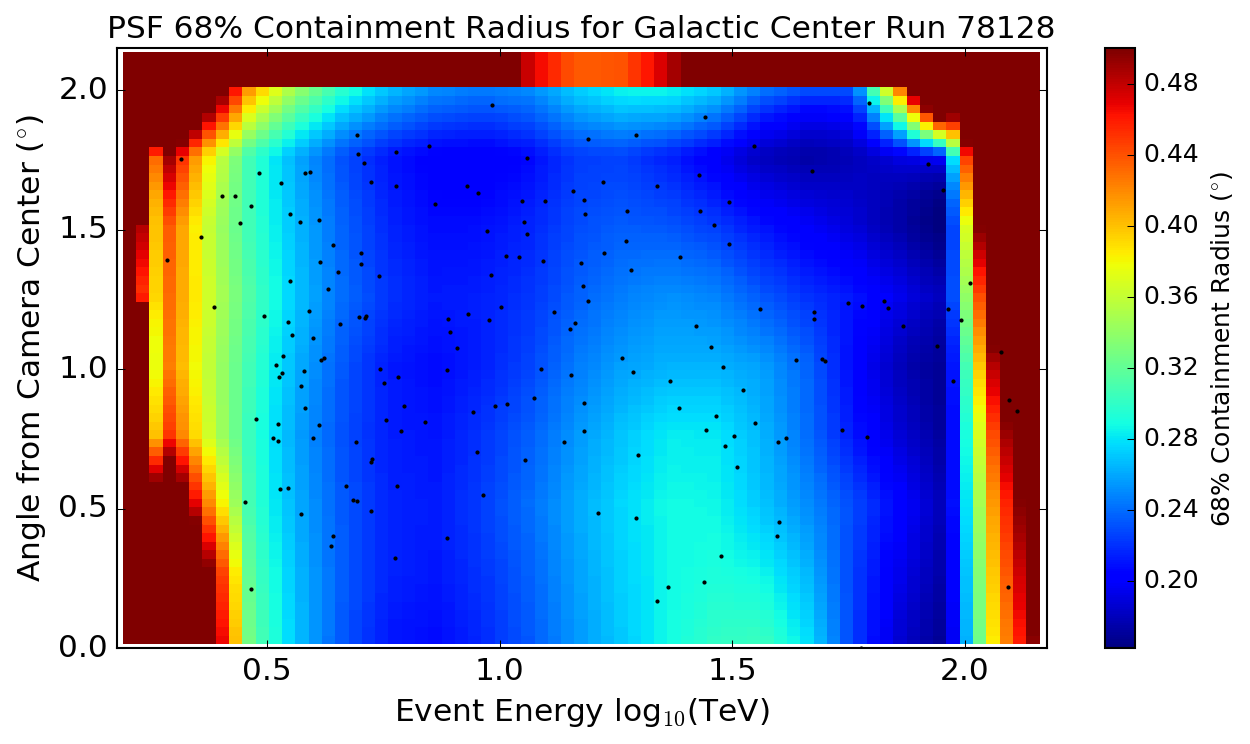
\includegraphics[width=0.85\textwidth]{images/psf_king_plots/psf_parameter_space.pdf}
      \caption[PSF Parameter Space]{
        The 68\% containment radius for the Energy/Offset parameter space for Sgr A* run 78128. 
        The green points are from data, showing a subset of the event locations from run 78128 in the parameter space.
        The color axis is the containment radius, calculated from simulations.
        While events from all energies are shown, only events from \SIrange{4}{70}{\TeV} are used (see Section \ref{sec:crab_analysis} {\color{red}(where is this section now!??)}).
      }
      \label{fig:psf_paramspace}
    \end{figure}

    For the Galactic Center and the Crab analyses, the distribution of 68\% containment radii for all events is shown in Figure \ref{fig:gc_psf_hist}.

    \begin{figure}[ht]
      \centering
      \includegraphics[width=0.85\textwidth]{images/psf_gc_eventhist/eventpsf.eps}
      \caption[Crab and Galactic Center Event PSFs]{
        The 68\% containment radius for all Galactic Center and Crab Nebula events used in this analysis.
        {\color{red}why the long tail?? Large offset and low energy data?? -Gernot}
        {\color{red}You need to explain in the text any non-trivial features in the plots. That is, you need to say what is the resolution observed and explain what is the second peak seen in the Galactic centre data. ?? -Orel}
        {\color{red}Crab -> Crab Nebula ??}
      }
      \label{fig:gc_psf_hist}
    \end{figure}
  
  \FloatBarrier
  
  \subsection{Background Models}\label{background_production}
  
    A background model is a 3 dimensional function in camera x (in angle, parallel to azimuth), camera y (in angle, parallel to elevation), and energy.
    Each background model is constructed from one of two templates, and the templates are built from dark run observations (see Figure \ref{fig:gcfieldsofview}).
    These background models calculate the number of expected events in the camera, per unit solid angle, unit time, and unit energy.
    This is used to quantify how many counts are expected in different parts of the camera when observing any target.
    Understanding the background shape of the camera is crucial for properly studying extended sources, like dark matter halos, which may extend several degrees from the Galactic Center.
    Improperly estimating background models can result in fake structures appearing around an astrophysical target.
    Background models with more than three dimensions are also possible, but require many more simulations, and are beyond the scope of this thesis.
    
    The background models used in this analysis are made from two background templates, one for each of the V5/V6 epochs (see Section \ref{sec:epochs}).
    The templates are constructed from dark observations, detailed in \ref{veritasdata}.
    Each template is made by histogramming all background events by their energy, dividing by the bin width, and interpolating between bins to produce a spectral function.
    This spectral function can be seen in Figure \ref{fig:background_profile}.
    
    {\color{red}These two paragraphs can be shortened to one short one with less details. Just mention the binning radially and in energy. The technical way it is done is of less interest. ?? -Orel}

    \begin{figure}[ht]
      \centering
      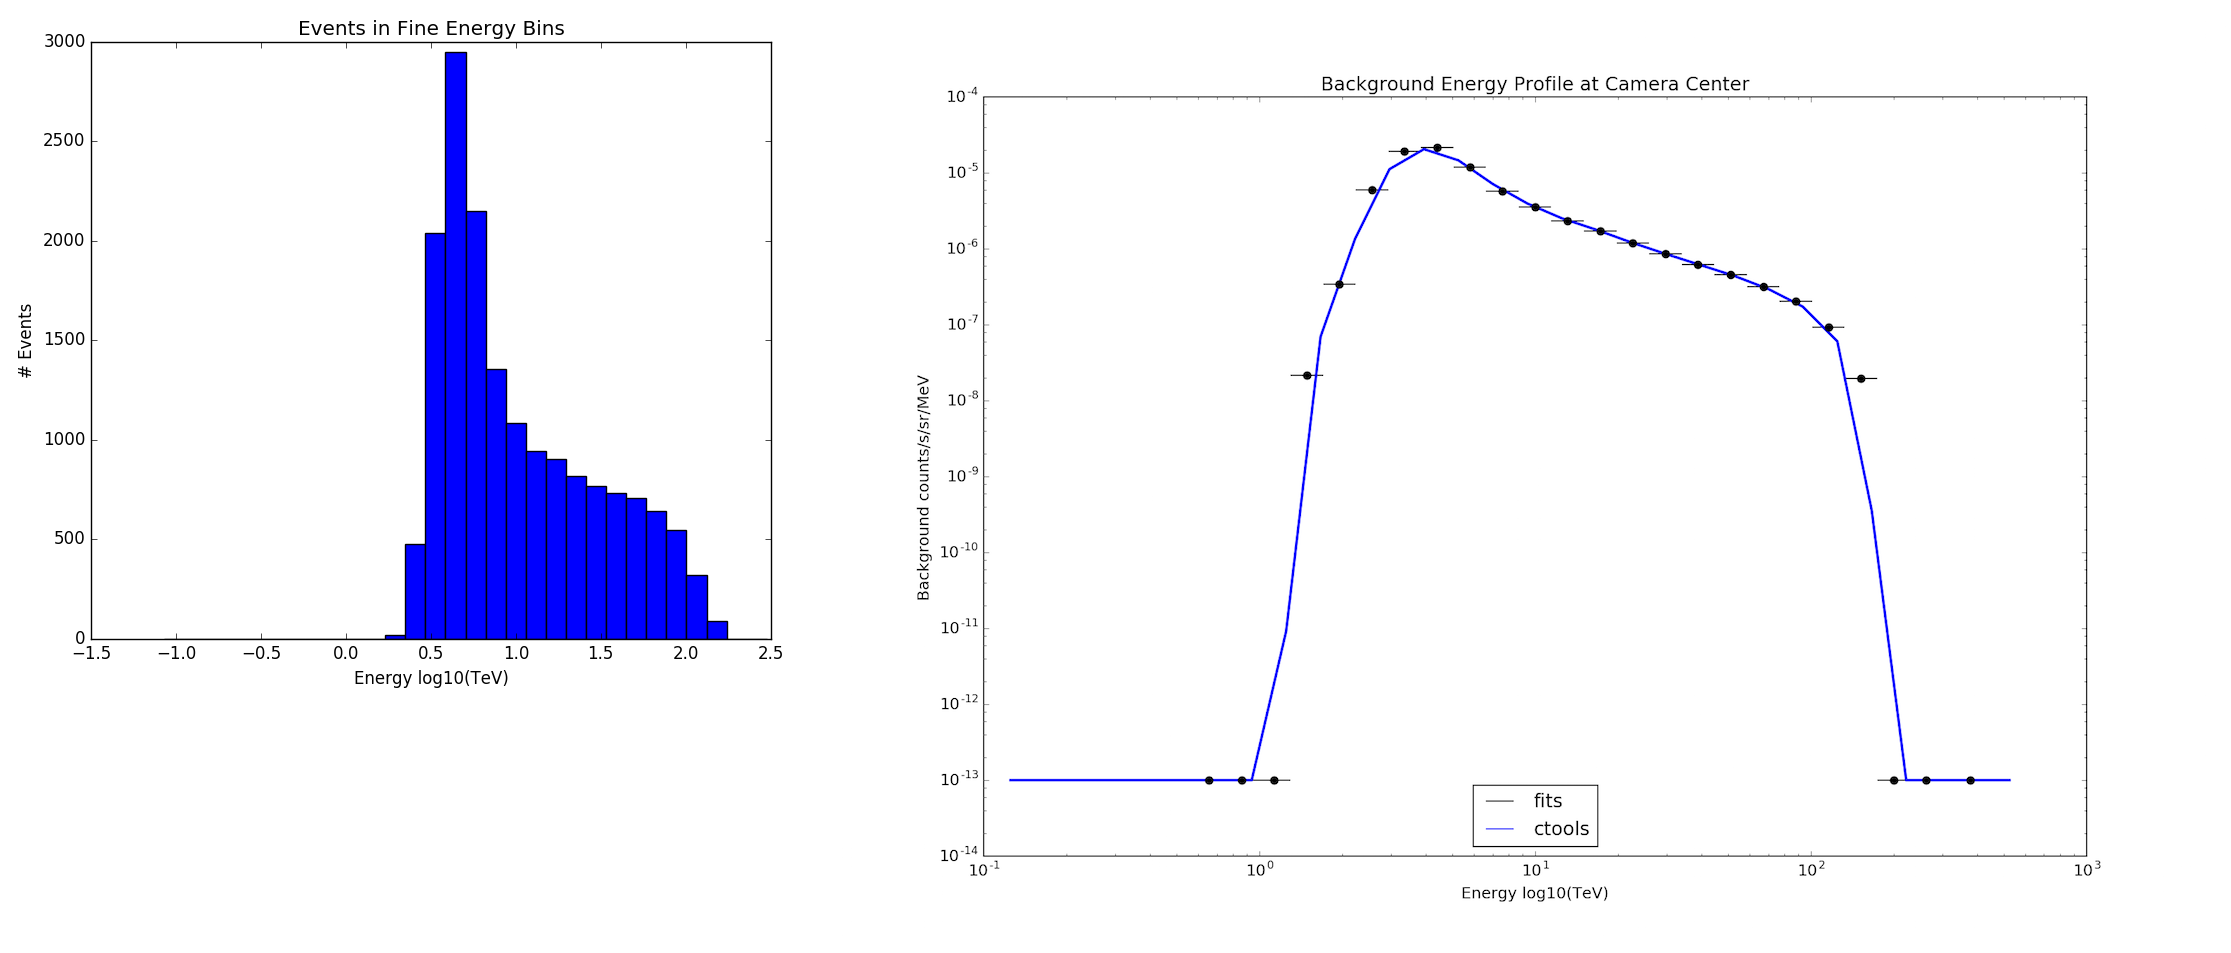
\includegraphics[width=0.65\textwidth]{images/ctools_background/background_construction.eps}
      \caption[CTOOLS Background Fine Energy Bins]{
        The V5 Background's fine energy bins.
        The top plot shows the number of events in each fine energy bin.
        The bottom plot shows the CTOOLS background values.
        The black lines show the fits background value and energy bin width saved to the background file, while the blue line shows the background value after CTOOLS loads and interpolates those fits background values.
        {\color{red}Please do not mention it as CTOOLS. Rather, write it in “physics language”, fit, background rate, etc. ?? -Orel}
        {\color{red}X axis labels should be consistant!??}
      }
      \label{fig:background_profile}
    \end{figure}

    Then, the events are divided into high and low energies, and the events' reconstructed camera positions are binned radially about the camera center, with each bin divided by its bin area, producing two spatial functions.
    These high- and low-energy spatial functions are shown in Figure \ref{fig:background_radial}.
    {\color{red}(tweak hyperref plugin to make links a different color??)}
    
    \begin{figure}[ht]
      \centering
      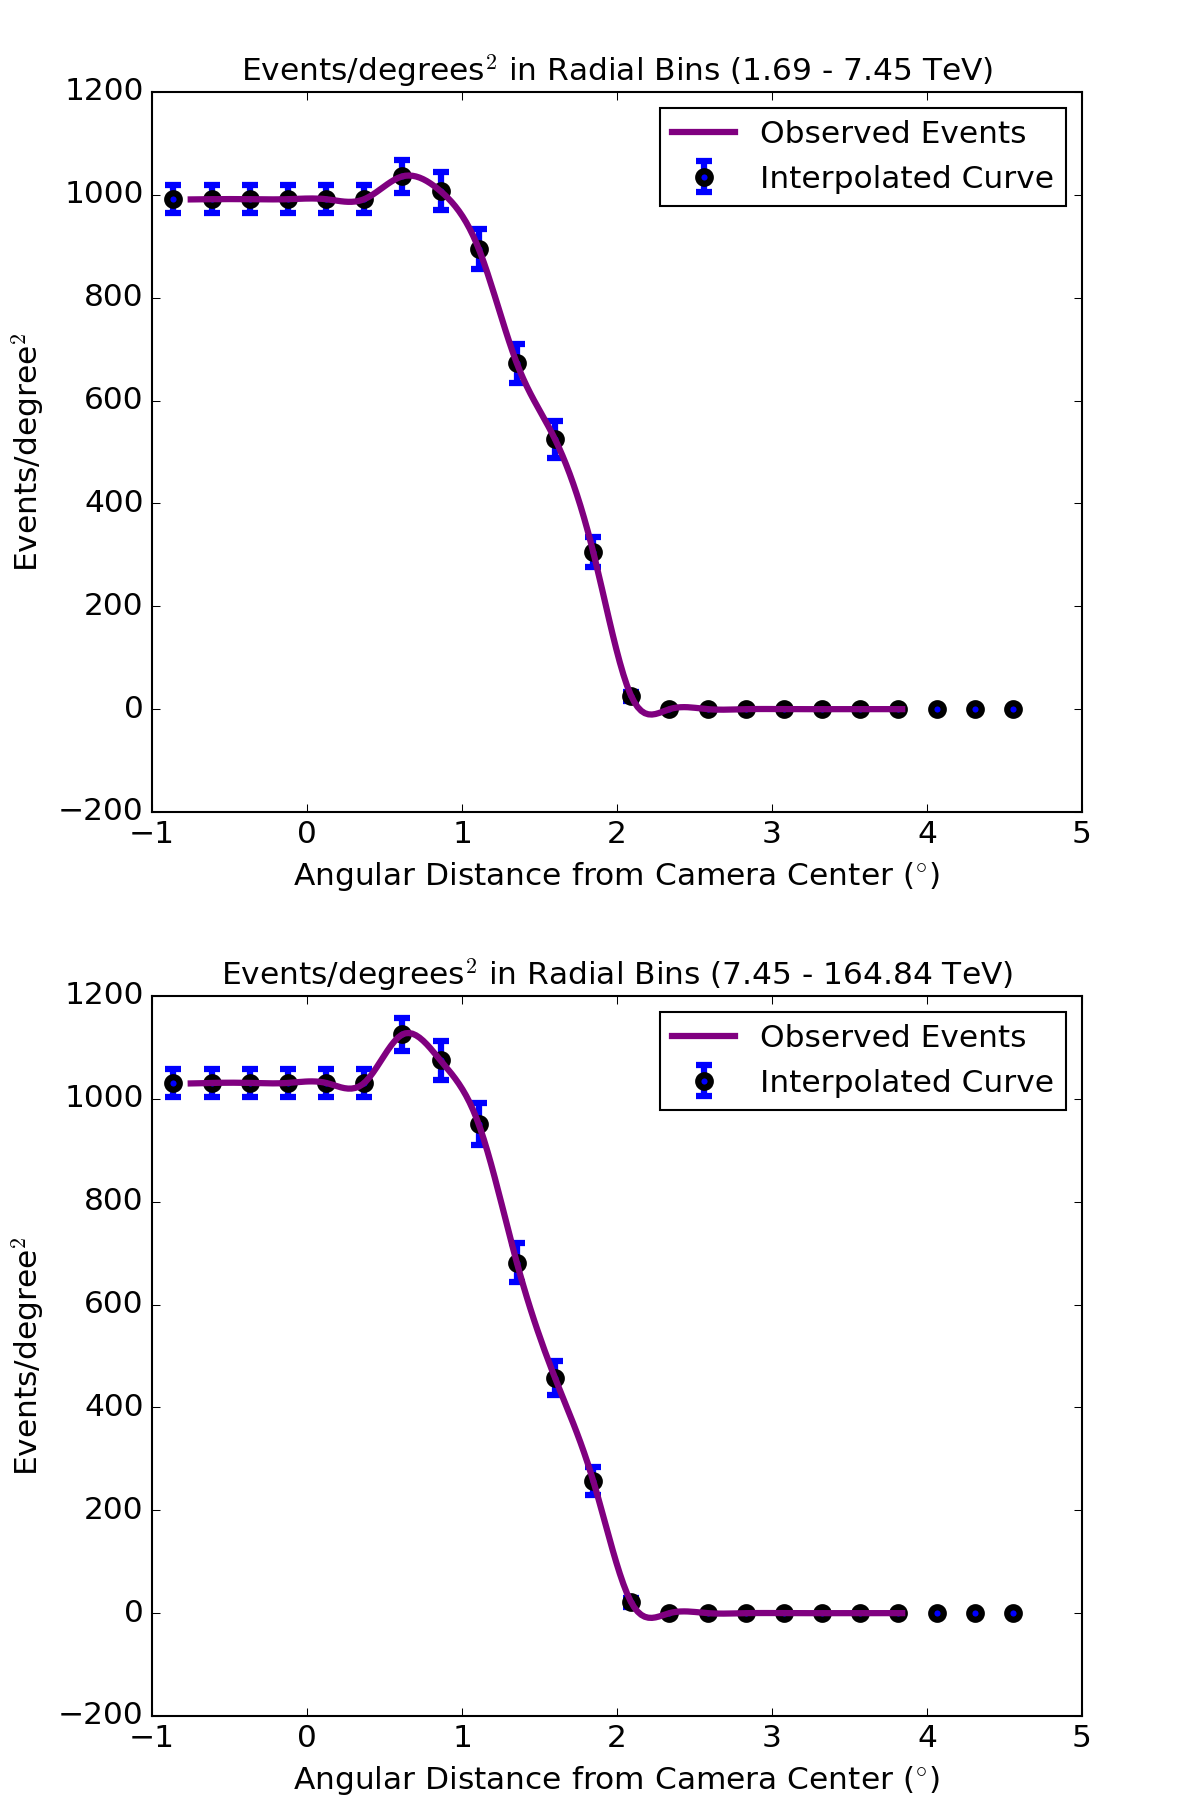
\includegraphics[width=0.65\textwidth]{images/ctools_background/radial_profiles.eps}
      \caption[CTOOLS Radial Background Profiles]{
        Radial bin profiles for the V5 background's two large-scale energy bins.
        The blue points are the counts per bin area, while the purple line is a spline interpolation with a 3rd order polynomial.
        {\color{red}You need to explain in the text the feature seen in both plots, the plateau and small peak at about 1 degrees. ?? -orel}
        }
      \label{fig:background_radial}
    \end{figure}
    
    Finally, the spatial and spectral functions are multiplied together, as in Equation \ref{eqn:bck_template}.
    
    \begin{equation}\label{eqn:bck_template}
      f(e,x,y) = A \times \textrm{spectral}(e) \times \textrm{spatial}(e,x,y) 
    \end{equation} 
    
    The function $f(e,x,a)$ has units of $\frac{\textrm{Number of Counts}}{ \textrm{MeV} \times \textrm{s} \times \textrm{sr} }$.
    The multiplied functions are then scaled with a constant $A$ such that the total integral of the template (integrating across camera x, camera y, and energy) is equal to the original number of counts in the dark runs, as in Equation \ref{eqn:background_template_function}.
    
    \begin{equation}\label{eqn:background_template_function}
      \textrm{Number of Background Events} = A \times \int \textrm{spectral}(e) \times \textrm{spatial}(e,x,y) \times dx \: dy \: de
    \end{equation}

    This function $f(e,x,y)$ is the background template in camera x/y, which due to its radial symmetry can then immediatly be used as a CTOOLS background model in RA/Dec.
    Each background template is used in the likelihood analysis as a model multiplied by two free parameters, a normalization factor, and the event energy exponentiated by the spectral index.
    This lets the likelihood fitter scale each run's background model up or down to best match the number of observed events.
    This means the background's absolute value is less important than the relative values in different parts of the camera background or at different energies.
  
  \FloatBarrier

  \subsection{Energy Dispersion}\label{subsec:edisp}
    As events are reconstructed imperfectly, it is important to understand what the distribution of true energies are for a given reconstructed energy.{\color{red}(Again, not sure, but perhaps the other way around?? -Orel)}{\color{red}(just remove all mentions of $f_{reco}$, its not necessary ??)}
    This \textit{dispersion in energy} is quantified by an energy migration matrix $E_{i,j}$, where $i$ denotes the $i^{\text{th}}$ reconstructed energy bin, and $j$ denotes the $j^{\text{th}}$ true energy bin.
    The energy migration matrix can be used to account for two significant effects.
    The first is that the reconstruction method introduces biases in the event energy, meaning an event at a given true energy can be reconstructed on average at a higher or lower energy.
    The second effect that is accounted for is the dispersion in the reconstructed energies.
    Gamma rays with the same energy will have their energies reconstructed as a distribution close to the true energy.
    These fluctuations can be due to randomness in air shower development or atmospheric absorption of Cherenkov photons.
    This has the effect of distributing events in each energy bin of a spectra.
    In the gamma-ray spectra of astrophysical sources, which often follow a power law, lower energy bins tend to have more events than higher energy bins.
    This results in lower-energy dispersion contributing more to the higher-energy bins than the higher-energy dispersion contributes to the lower-energy bins.
    When not accounted for, this has the effect that the energy dispersion will harden observed astrophysical spectra.
    In Figure \ref{fig:migmatrix}, a migration matrix is shown.

    \begin{figure}[ht]
      \centering
      \includegraphics[width=0.85\textwidth]{images/edisp_plots/edisp.eps}
      \caption[Energy Migration Matrix]{
        An energy migration matrix used with Sgr A* run 82288.
        The reconstructed energy is on the x axis, and the true energy is on the y axis.
        The z (color) axis denotes the number of simulated events that passed all cuts.

        {\color{red} (why does the z axis have units of 1/s*MeV?? GCTAEdisp2D::operator() returns these units, but why??)} 
      
        {\color{red}Most events are reconstructed off axis?? -Gernot}
        
        {\color{red}Need to explain downturn at lowest energies?? -Gernot}
        
        {\color{red}Again, please describe in the text non-trivial features in the plot (the bias at low energy) ?? -orel}
      }
      \label{fig:migmatrix}
    \end{figure}
  
  \FloatBarrier

\section{Camera Studies}
  The objective of this thesis is to put upper limits on the existance of a gamma-ray source that is both extended and faint.
  {\color{red}(That is not the objective of the analysis though. The objective is to search for dark matter, not to admit defeat from the get go and aim at setting an upper limit.?? -Orel) (This sounds like you've already admitted defeat before the analysis started, your object should be to find dark matter, win a nobel prize!??)}
  In order to better understand the effects that may impact the VERITAS camera behavior in the reconstruction method, several studies were performed.
  {\color{red} You should connect between these two sentences, “because it is extended and faint, the background has to be determined with high precisions, etc.” ?? -Orel}

  \subsection{Background Structure at the Low Energy Threshold}
    To produce background models, events were binned according to their energy, elevation, and camera x and y coordinates.
    As a result of this detailed binning, some new effects were noted.
    First, a series of gamma-like events were selected from observations with no known gamma-ray sources.
    These events were then divided into equal-statistics energy bins.
    For each bin, all the contained events were then binned in camera x and y.

    For a set of high-elevation observations, these backgrounds are shown in Figure \ref{fig:back_highelev}.
    It can be seen that all events are divided up into 3 equal-statistics energy bins in Figure \ref{fig:back_highelev}.A.
    Each energy bin is then binned in camera x and y in Figures \ref{fig:back_highelev} B, C, and D.
    At these high elevations, the distribution of events in each energy bin is radially symmetric about the camera center.
    This happens because the gamma ray's point of origin, and its shower image in the camera, are usually several tenths of a degree away from each other.
    In addition, the atmospheric column density is similar in all parts of the camera.
    However, structures start to break the radial symmetry at low energies and elevations.
    The cause of these structures is explored in Section \ref{subsubsec:diffusesims}.

    \begin{figure}[ht]
      \centering
      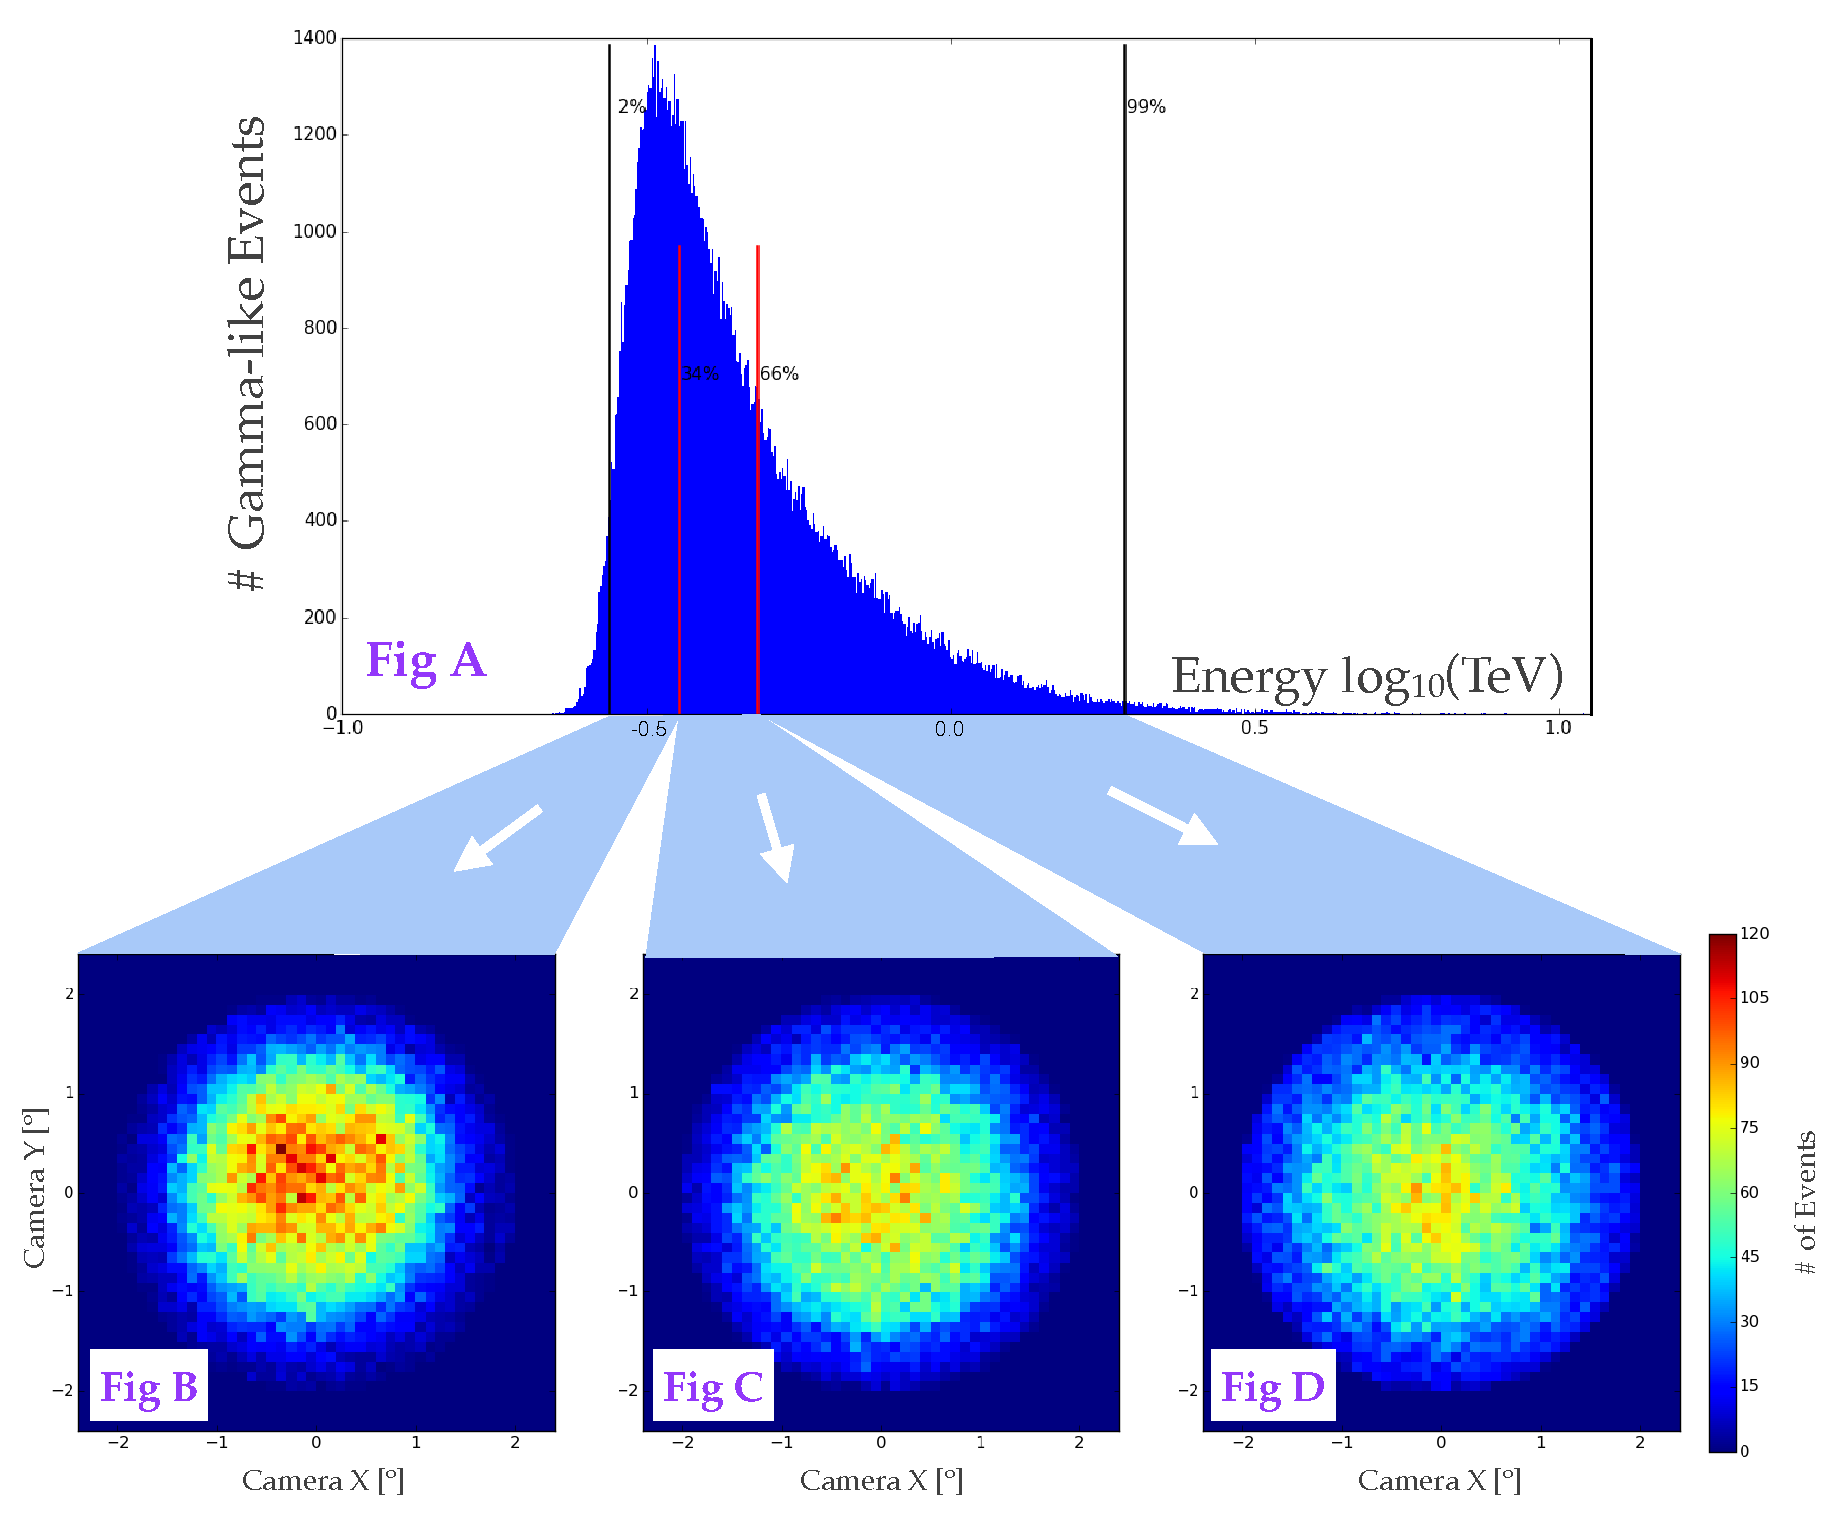
\includegraphics[width=\textwidth]{images/ctools/backgrounds_highelev.eps}
      \caption[FITS Background at \ang{50} Elevation]{
        Gamma-like Events from 52 observations (approximately \nicetilde20 hours) of M82, between \ang{50} and \ang{52} elevations.
        Events in Figure A are divided into 3 equal-statistics energy bins, and binned in Camera Coordinates in Figures B, C, and D.
      }
      \label{fig:back_highelev}
    \end{figure}

    In Figure \ref{fig:back_lowelev29} and Figure \ref{fig:back_lowelev26}, the same plots are constructed for a set of low-elevation (\nicetilde{}\ang{29} and \nicetilde{}\ang{26} respectivly) observations, using dark observations.
    See Section \ref{background_production}, Figure \ref{fig:gcfieldsofview}, and Section \ref{sec:bkgmodels} for more discussion.
    It can be seen that in different energy bins, the background possesses different shapes.

    \begin{figure}[ht]
      \centering
      \includegraphics[width=\textwidth]{images/ctools/backgrounds_lowelev29.eps}
      \caption[CTOOLS Background at \ang{29} Elevation]{
        15 Sagittarius A* Off runs (\nicetilde7.5 observation hours), between elevations $ \ang{27.5} $ and $ \ang{30} $.
        Events are divided into 6 equal-statistics energy bins, of which four are binned in Camera Coordinates in Figures B, C, D, and E.
      }
      \label{fig:back_lowelev29}
    \end{figure}

    \begin{figure}[ht]
      \centering
      \includegraphics[width=\textwidth]{images/ctools/backgrounds_lowelev26.eps}
      \caption[CTOOLS Background at \ang{26} Elevation]{
        10 Sagittarius A* Off runs (\nicetilde5 observation hours), between elevations \ang{24} and \ang{27.5}. 
      }
      \label{fig:back_lowelev26}
    \end{figure}
  
  These effects are also noticeable in the galactic (l,b) event maps.
  In Figure \ref{fig:bkgvsel_crab}, the top plot shows the positions of all events.
  The middle histogram shows the distribution of event energies, and the bottom plot shows the positions of events in a limited energy range, \SIrange{1.5}{3.25}{\TeV}.
  The middle plot demonstrates that, as event energy decreases, fewer events are detected.
  When events in this limited energy range are plotted in the bottom plot, a faint deficit appears along the bottom of the camera.
  This faint deficit is due to the \nicetilde20\% higher column density at the low-elevation parts of the camera.
  This higher column density causes air showers to start farther away from the telescopes, where more Cherenkov photons are absorbed, resulting in fewer events being detectable in the lower half of the camera.

  When similar plots are made for the Galactic Center in Figure \ref{fig:bkgvsel_sgra}, the effect is much stronger, and rotated.
  In the top plot, events are radially symmetric around the source position.
  When only the events from \SIrange{1.5}{3.25}{\TeV} are plotted, a much clearer deficit is visible on the lower right part of the plot.
  This area corresponds to the deficit at the bottom of the camera in Figures \ref{fig:back_lowelev29}.B and \ref{fig:back_lowelev26}.B.
  This rotation occurs when converting between camera x/y coordinates (Earth Elevation/Azimuth) and Galactic coordinates (l,b).
  The degree of rotation also changes throughout individual runs, which further blurs this effect.
  For the Crab plots in Figure \ref{fig:bkgvsel_crab}, the rotation is only a few degrees, while for Sgr A* in Figure \ref{fig:bkgvsel_sgra}, it is closer to \ang{70}.
  
  This effect is important to the analysis because it implies that, at the lowest energies, the background rate is not radially symmetric.
  Radial backgrounds (sometimes referred to as acceptances) are typically used in VERITAS, as no other camera x/y or energy dependence had been demonstrated until now.
  As the analysis in this thesis only has a few hours of background observations (see Table \ref{tab:observation_times}), only radially symmetric background templates and models could be constructed, which then required limiting the final analysis to $\geq\SI{4}{\TeV}$.
  
  \begin{figure}[ht]
    \centering
    \includegraphics[height=0.9\textheight]{images/background_vs_elevation/background_vs_elevation_srccrab.eps}
    \caption[Background Vs Elevation Crab]
    {\small 
      Plots of Crab Nebula observations.
      Top: Skymap of all events.
      Middle: Histogram of all events in energy.
      Bottom: Skymap of events from \SIrange{1.5}{3.25}{\TeV}.  
      The blue circles centered on the Crab Nebula highlight the radial symmetry of the top plot, and the lack of radial symmetry in the bottom plot.
      {\color{red}(Add high energy plot??)}
    }
    \label{fig:bkgvsel_crab}
  \end{figure}

  \begin{figure}[ht]
    \centering
    \includegraphics[height=0.9\textheight]{images/background_vs_elevation/background_vs_elevation_srcsgra.eps}
    \caption[Background Vs Elevation Sgr A*]
    {\small 
      Plots of Sgr A* observations.
      Top: Skymap of all events.
      Middle: Histogram of all event energies.
      Bottom: Skymap of events from \SIrange{1.5}{3.25}{\TeV}.  
      The blue circles centered on the Galactic Center highlight the radial symmetry of the top plot, and the lack of radial symmetry in the bottom plot.
    }
    \label{fig:bkgvsel_sgra}
  \end{figure}
  
  \FloatBarrier

  \subsection{Diffuse Simulations}\label{subsubsec:diffusesims}
    Diffuse simulations were performed at similar energies and elevations to see if this effect was still present.
    These consisted of simulating 50,000 gamma rays with CORSIKA (\cite{corsika1998}) at 1.4, 1.6, 2, and \SI{5}{\TeV}.
    The telescopes were fixed to an (azimuth,elevation) of (\ang{193}, \ang{28}).
    The events themselves were distributed in a diffuse \ang{2.5}-radius disk.
    To approximate a simple gamma-hadron cut, any events with a mean-scaled-width falling outside the range of -2.0 to 0.5 were removed, which eliminates many of the showers that appear proton-like.
    These remaining 'gamma-like' events are then binned in camera coordinates in Figure \ref{fig:back_simdiffuse}.

    \begin{figure}[ht]
      \centering
      \includegraphics[width=\textwidth]{images/backgrounds_diffuse_vs_data/backgrounds_sims/backgrounds_sims.eps}
      \caption[Diffuse Simulated Backgrounds]{
        Diffuse simulated gamma-like events in the camera coordinate system at a \ang{28} elevation, at 4 different initial energies.
        {\color{red}What does the True camera position look like for these events??}
      }
      \label{fig:back_simdiffuse}
    \end{figure}

    The ring and crescent structures persist in these diffuse simulations, implying these are physical effects of the atmosphere and camera, rather than a problem with the reconstruction method.
    {\color{red}(But what is the effect? I remember Gernot mentioning something about an edge effect? You should explain it here. --Orel??)}
    {\color{red}(The top-of-camera vs bottom-of-camera differences are due to the atmosphere, but I'm not sure what causes the deficit in the middle at the lower energies... ??)}
    {\color{red}(I am not sure what is the reason for the deficit in the middle. Are simulations always with a wobble? Maybe the showers are very small and always at some distance from the centre of the camera?? -Orel)}
    {\color{red}(Consider playing with the distribution of disps and the radial areas??)}

    This striking effect can be seen in the Galactic Center data in Figure \ref{fig:bkgvsel_sgra}.
    These structures, and their strong dependency on both the energy and elevation of the telescopes may be a large factor in why the low-energy threshold regime of gamma-ray telescopes is poorly understood.
    Incorporating this effect into the instrument response functions would require modifying Eventdisplay and CTOOLS, as well as creating another batch of diffuse simulations with elevation increments smaller than \ang{5}, all of which are computationally expensive.
    {\color{red}It is good to explain that this is a global issue and even suggest how it can be fixed generally for VERITAS, but do not mention the software packages or computationally expensive. Instead, write something like “background templates are needed for the different bins” and that it is beyond the scope of this analysis (or that it was not performed due to time constraints). ?? -Orel}
    {\color{red}(Since there isn't enough background runs to make properly elevation and energy dependent background models (see significance skymap in chapter 6), This should be phrased as "More data is needed to properly populate the increased number of bins." ??)}
  
  
  {\color{red}(discuss figure \ref{fig:bkg_diagram} more!??)}

  \begin{figure}[ht]
    \centering
    \includegraphics[width=\textwidth]{images/background_template/background_template.pdf}
    \caption[Background Phenomenology]{
      How the elevation gradient affects the background rate.
      Relative to the peak energy for an observing run, lower energy events will be detected more at the top of the camera.
      Events higher than the peak energy will be detected closer to the bottom of the camera.
      Behavior may also depend on the number of telescopes observing the event, or the specific telescope combination.
      {\color{red}(more??)}
    }
    \label{fig:bkg_diagram}
  

  \end{figure}
  \FloatBarrier

  \subsection{Effect of Stars}
    Understanding the camera's background is important for accurately modeling extended sources like dark matter halos.
    The camera's background shape is due to the performance of many individual camera pixels working together.
    VERITAS onsite operators had, in the past, noted that for apparent visible magnitude $m_V :$ 6-8 stars, the camera pixels they illuminated would have a higher average current.
    This causes higher pedestal variations in the affected pixels, which decrease how often the pixel participated in shower images.
    In addition, if a star with $m_V < 6$ was in the field of view, it would cause a high enough current in the pixel to trigger a safety system that lowers its voltage to zero, to prevent it from being damaged.
    For particularly bright stars, such as $m_V \leq 3$, several pixels can be disabled at any given time.

    Compounding this effect is that, since the telescope camera is fixed to the ground, the sky rotates around the camera center.
    This means that over a single 30 minute observation the field of view rotates around the camera center, and each star in view disables successive camera pixels as it passes over them.
    The camera rechecks these disabled pixels roughly once per minute by turning their voltage back on and monitoring the current, and resetting it to zero if the current is still above the threshold.

    These effects imply that to study the effect of stars, one must study the effect of high-current and disabled camera pixels, and use this information to construct the effect of stars.
    In the following section, the effects of disabled camera pixels are studied.
    
  \subsection{Effects of Disabled Pixels}

    % see calculations/disabledpixel_obstime , those 250 crab runs turned into about 13.5 observation hours
    To examine the effects of disabled pixels, \nicetidle13 hours of Crab observations were reconstructed twice.
    The first analysis was with the default analysis chain settings, and the second time with a single pixel disabled in all four telescopes.
    This mimics the effect of having a star in the field of view that is bright enough to disable a pixel.

    After gamma-hadron cuts are applied to both sets of events, studies can be performed on events that only appeared in one set and not the other.
    Some events may only pass gamma-hadron cuts with the pixel enabled ($P_e$), while others only pass when the pxiel is disabled ($P_d$).
    Events that are present both when the pixel is disabled and enabled can also be tested to see how far their reconstructed position moved in the camera.

    In Figure \ref{fig:dpix_rel_camera}, the relative event rate in the camera is plotted when pixel 115 is disabled in all four telescopes.
    This relative event rate is calculated by binning all $P_d$ and $P_e$ events by their reconstructed position in camera coordinates.
    Then, for each camera coordinate bin, the ratio of the number of events $\frac{P_d}{P_e}$ is calculated.
    It can be seen that there is a loss of events near the disabled pixel (the black circle), with a rate closer to 100\% the farther one goes from the disabled pixel.

    \begin{figure}[ht]
      \centering
      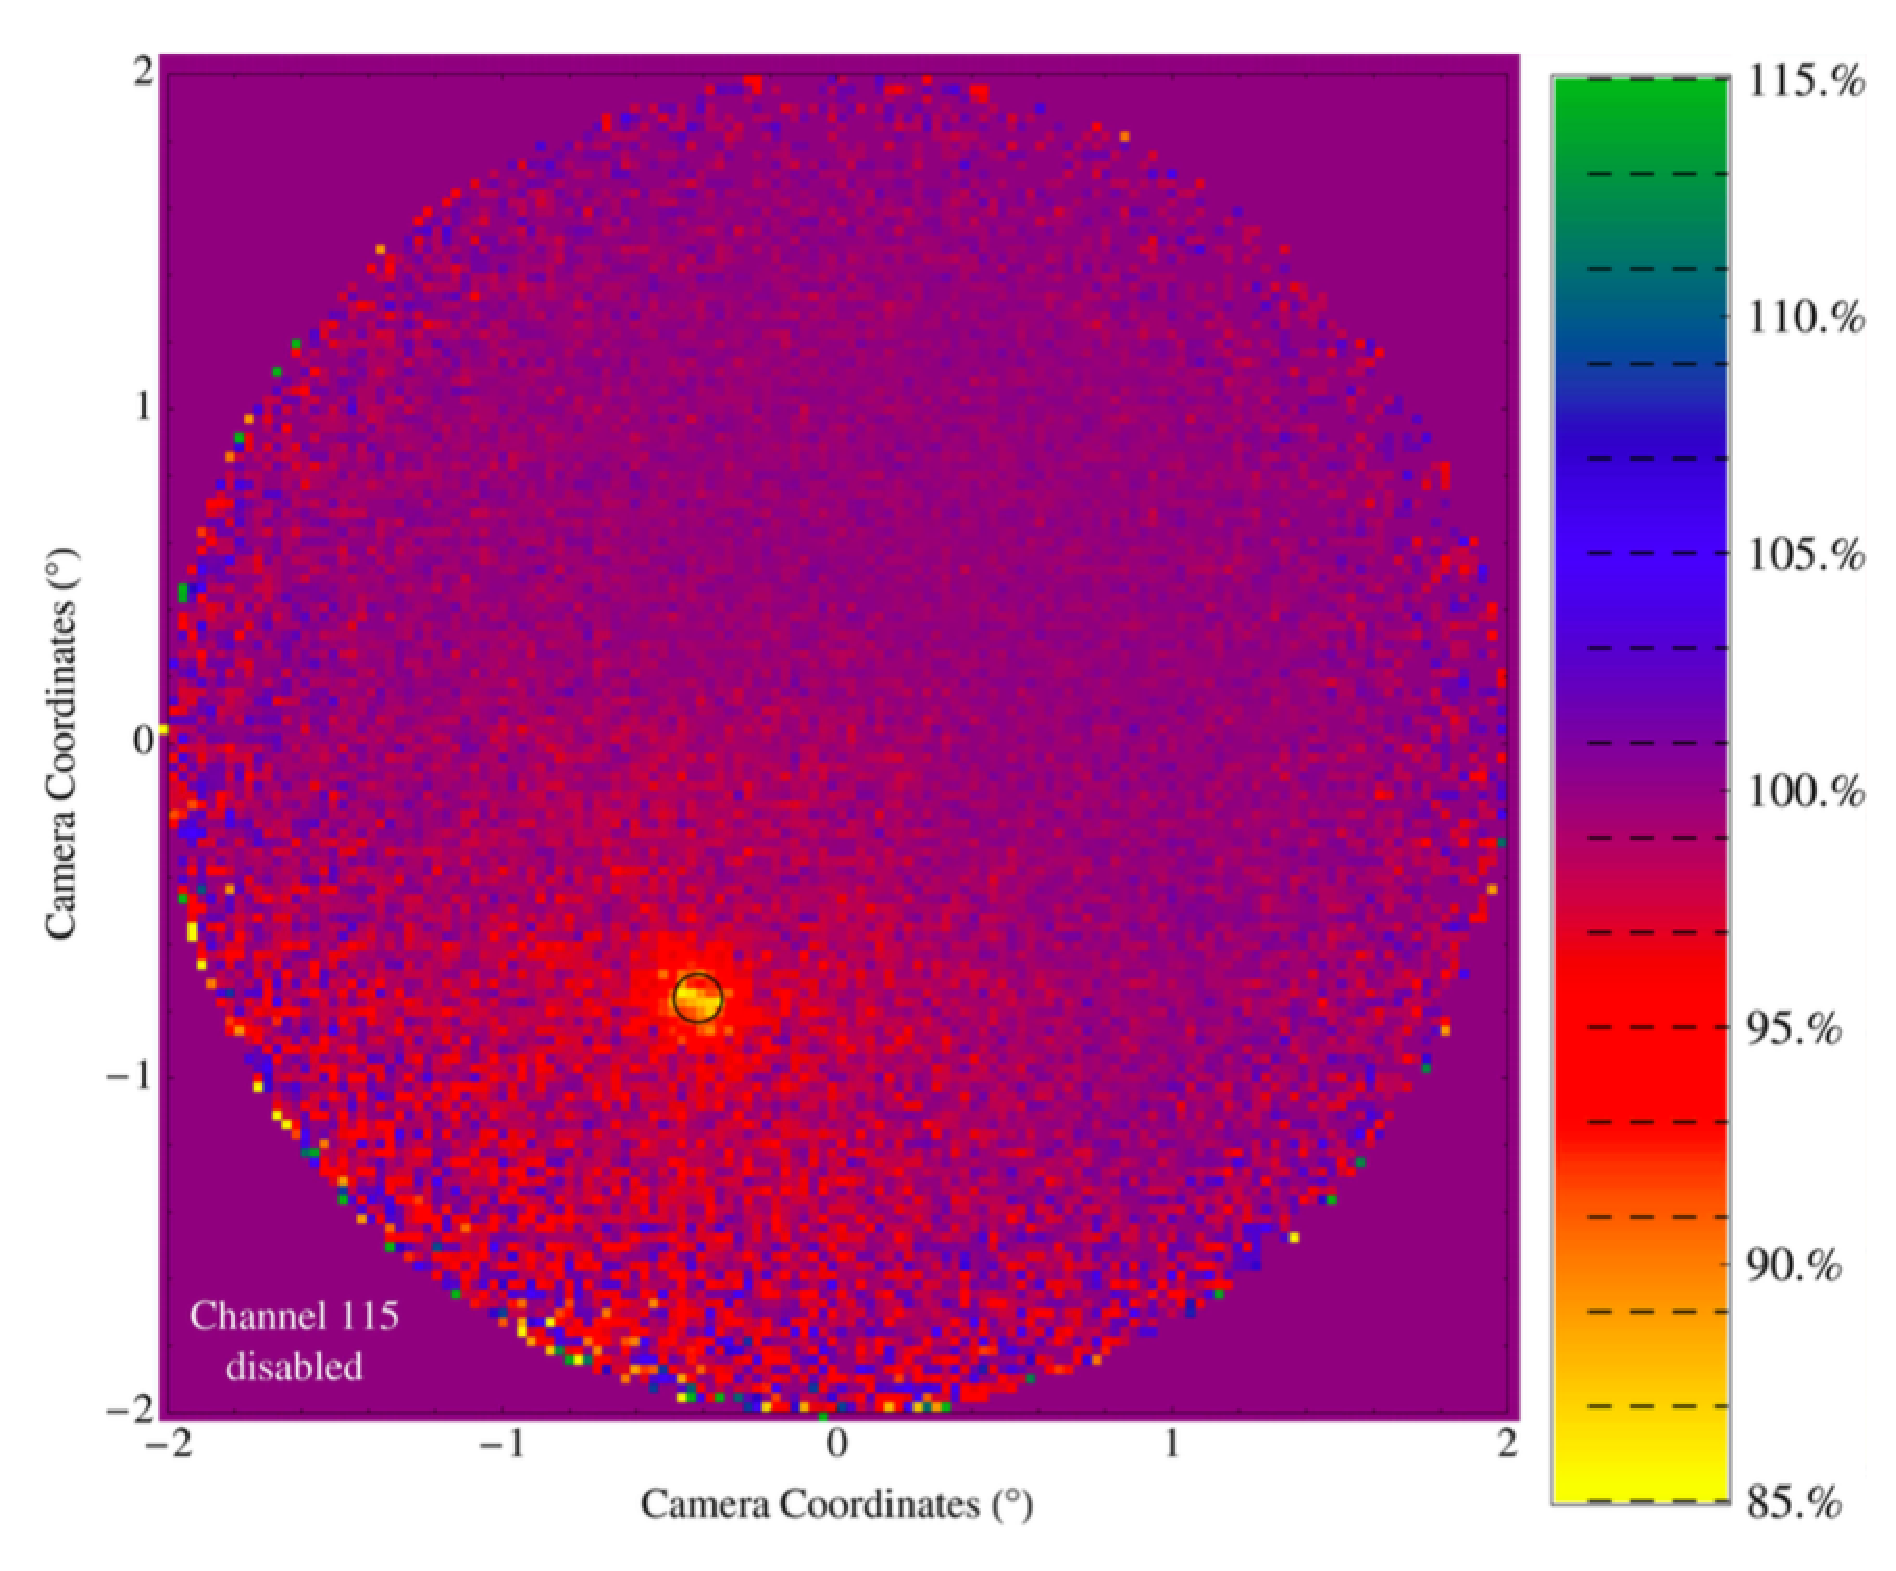
\includegraphics[width=0.8\textwidth]{images/disabled_pixel/relativerate_camera}
      \caption[Relative Event Rate]{
        Event rate in the camera with pixel 115 disabled (denoted by the black circle) in all four telescopes, relative to having all pixels enabled.
        Camera coordinate axes are parallel to azimuth and elevation.
      }
      \label{fig:dpix_rel_camera}
    \end{figure}
    
    While this single-pixel loss-of-events effect was notable, it was not incorporated into the main analysis of this thesis due to the small effect it would have, compared to the amount of work it would take to implement.
    Future analyses may be able to account for these effects in their models of the background rates and effective areas.
    
    {\color{red}You should be a bit more careful how you write paragraph. You can say that the effect was determined to be small for your particular analysis, but you need to back this up with numbers. 
Try to estimate (back of the envelope calculation) what is the fraction of events you lose due to stars in your specific galactic centre observations. Consider that you lose about 5\% of the events in a circle of about \ang{0.3} around a star. So how many stars would you expect which would disable pixels, what is the fraction of events that would fall in that area, etc. 
I am sure that if you do this calculation you can estimate that the effect is much smaller than the statistical/systematic uncertainties and then it is justified to neglect. ?? -Orel}

    In Figure \ref{fig:dpix_disappear}, the positions of events that were rejected by cuts are shown.
    The white area indicates many events are lost in the area of the disabled pixel.
    These events would have smaller images, and would be much more susceptable to being cut.

    \begin{figure}[ht]
      \centering
      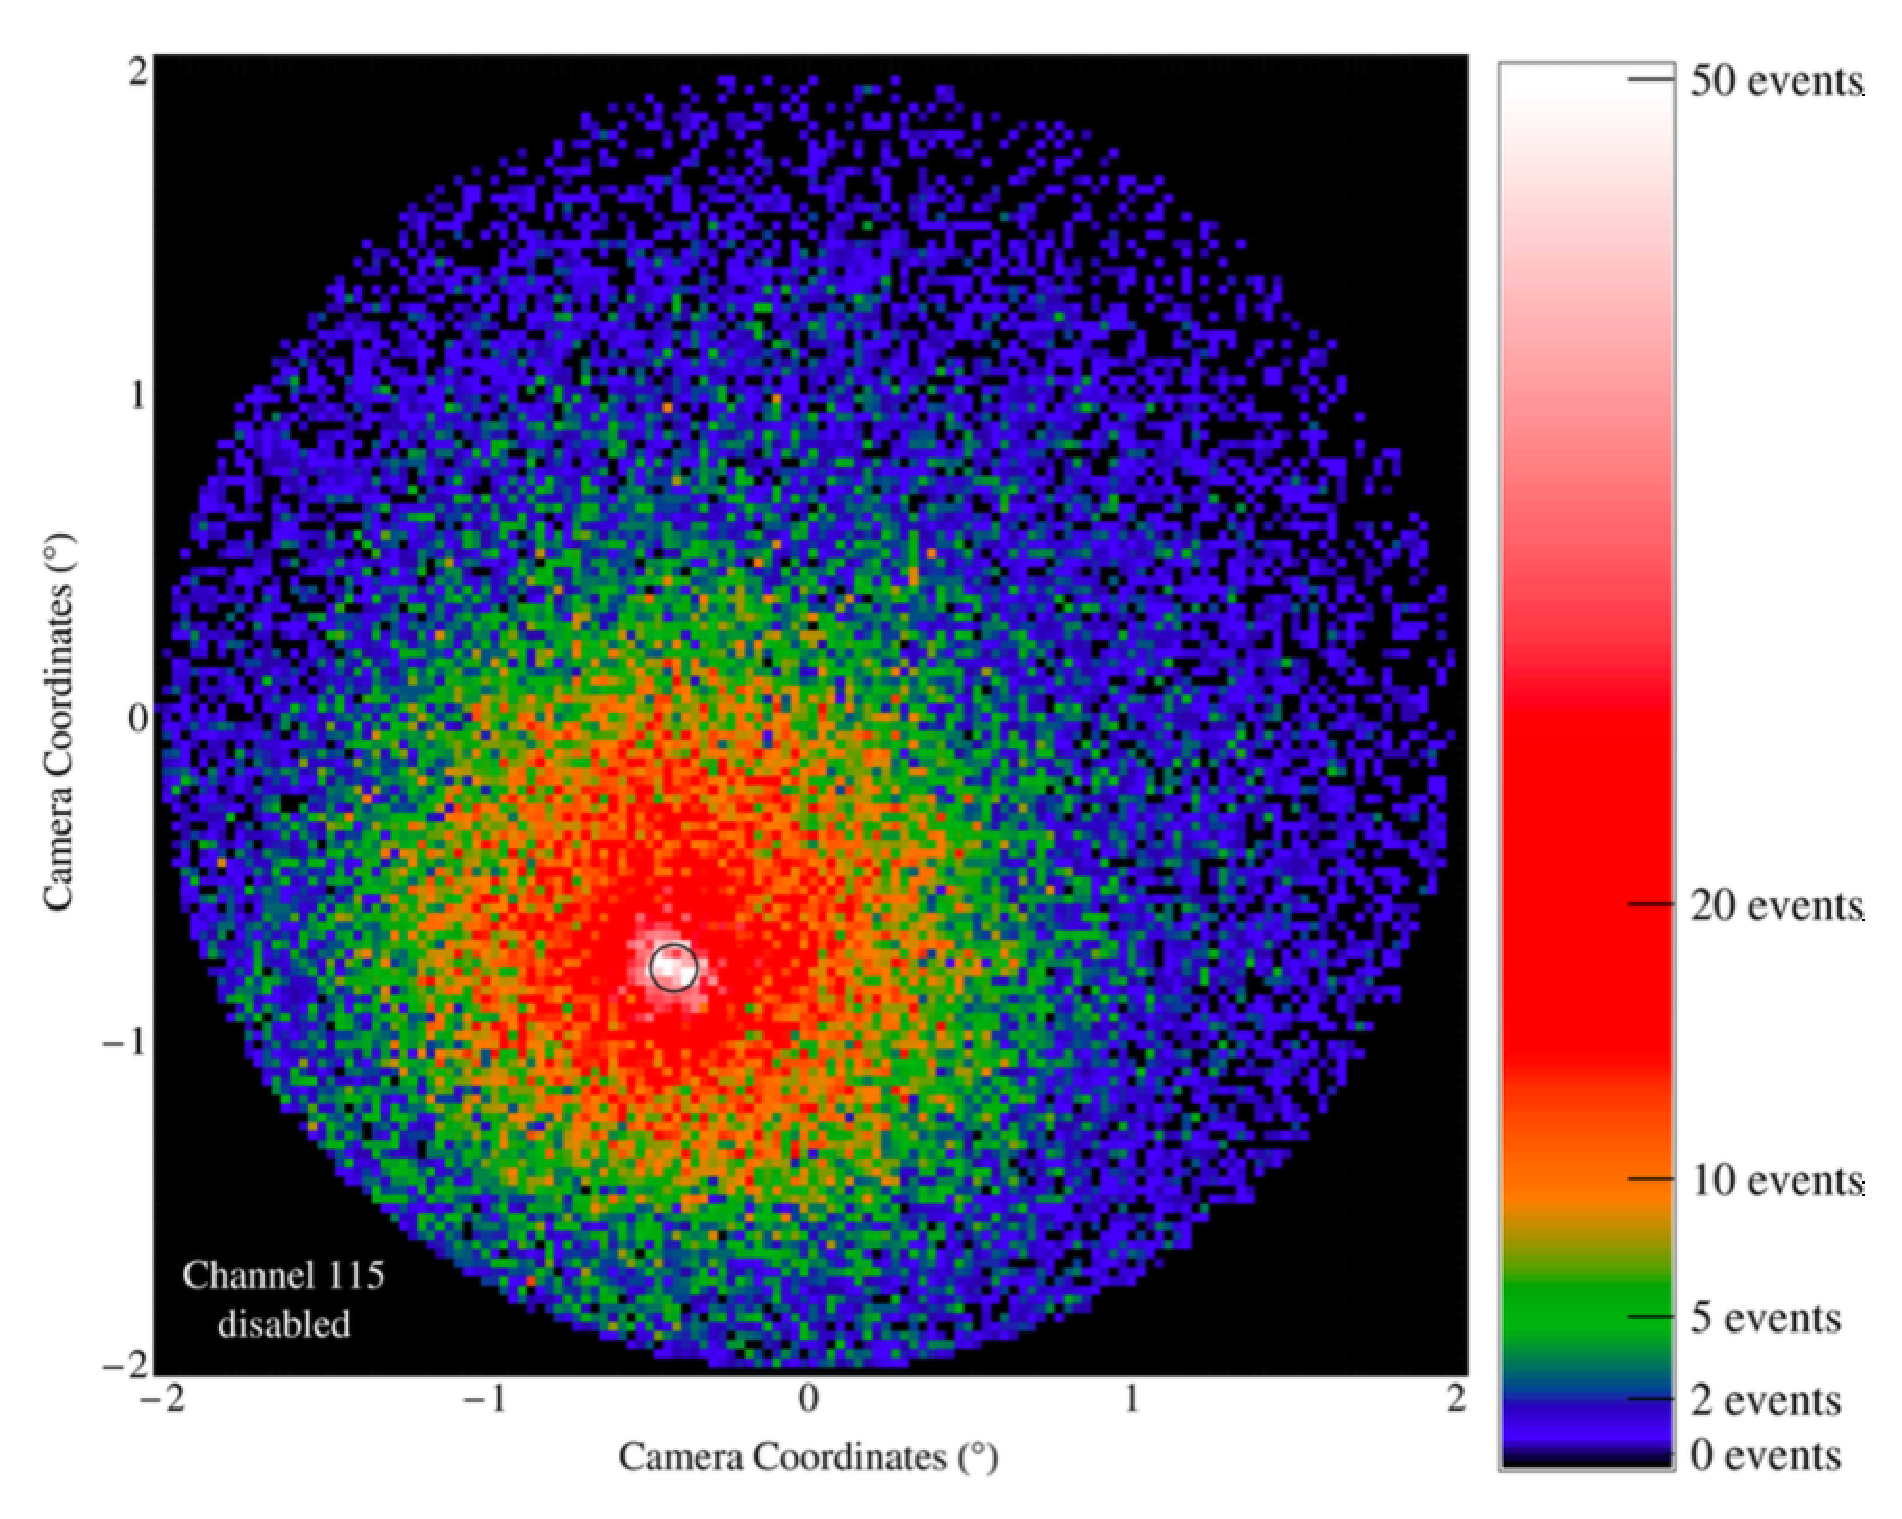
\includegraphics[width=0.8\textwidth]{images/disabled_pixel/disappearing_events}
      \caption[Disappearing Events]{
        Positions of events that disappeared when pixel 115 was disabled in all four telescopes.
        Positions are from their pixel-enabled reconstructed position.
      }
      \label{fig:dpix_disappear}
    \end{figure}

    In Figure \ref{fig:dpix_appear}, the positions of events that are now able to pass cuts are shown.
    It should be noted that these are not events that were 'created' by disabling a pixel.
    Rather, they are events that, with the pixel enabled, did not pass cuts.
    Now that the pixel is disabled, they do pass cuts.

    What is also noticeable is that the highest concentration of lost events was in the pixel's area, whereas the highest rate for appearing events is actually in a ring with a radius of \nicetilde1.5 pixels around the disabled pixel.
    This is probably due to the fact that disabling a pixel can make some images look thinner or wider, depending on where the disabled pixel is in the image.
    A thinner image will look more gamma-like, making it more likely to pass cuts.
    On the other hand, a wider image looks more hadron-like, and is less likely to pass cuts, causing some events to disappear.

    \begin{figure}[ht]
      \centering
      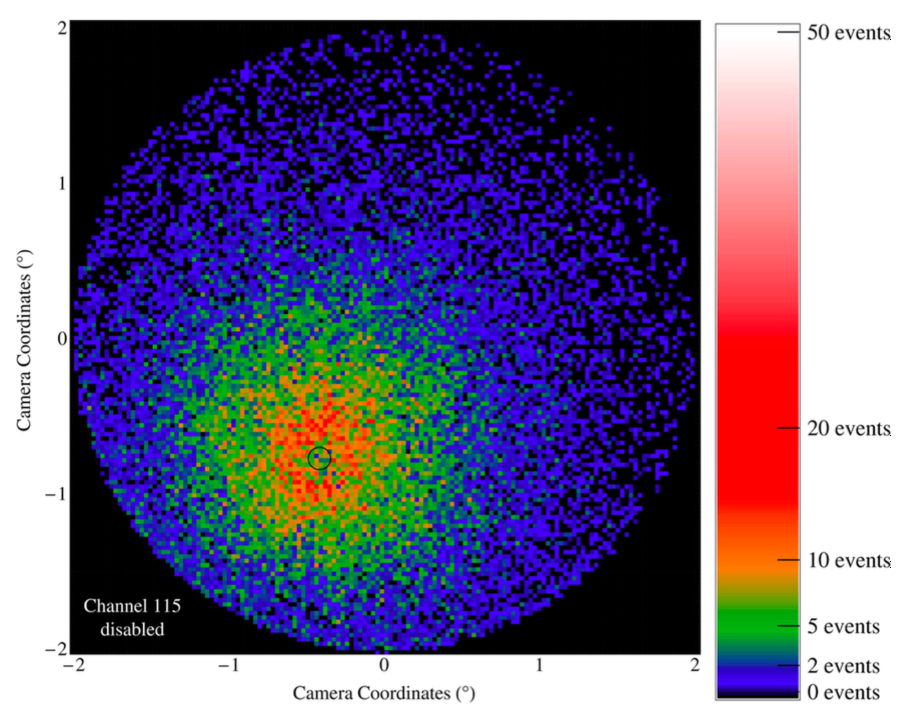
\includegraphics[width=0.8\textwidth]{images/disabled_pixel/appearing_events}
      \caption[Newly Appearing Events]{
        Positions of new events that appeared when pixel 115 was disabled in all four telescopes.
        Positions are from their pixel-disabled reconstructed position.
      }
      \label{fig:dpix_appear}
    \end{figure}

    In Figure \ref{fig:dpix_move}, the movement of gamma-like events is shown, when pixel 115 was disabled in all four telescopes.
    Only events which moved more than $0.1*\text{PSF}$ are shown.
    It should be noted that relatively few ( {\color{red}\nicetilde{}100 in the 20-minute-long run 53703 events} move more than this, and the events that do move are mostly ones with non-compact image shapes that are amputated when a pixel is disabled.
    {\color{red}(How many events are there in a 20 min run? People outside of VERITAS (and me) do not know the event rate so 100 can be 10\% or 0.1\% ??)}
    {\color{red}(Run 53703's datafile was deleted, and I don't have any other crab runs with soft cuts to estimate the event rate for a 20 minute run :(, see /afs/ifh.de/user/n/nkelhos/scratch/Effect\_Of\_Near\_Stars/Pixel\_Off\_Effect for more info ??)}

    {\color{red}(The conclusion in this paragraph is confusing. From the previous paragraph I thought that this effect is actually negligible for VERITAS. But this paragraph talks about effects of pixels halfway across the camera. If it is negligible, state it clearly and say that what is shown in the figure are those rare cases where the effect is noticeable.)}
    What can be learned from this is that while only a small number of events' positions depend on a given pixel, pixels can have an impact on the reconstructed position from halfway across the camera.
    This may imply that the event PSF is, to second order, dependent on the number of disabled pixels {\color{red}(Really? Could the PSF depend on the pixels? I thought it is only an optical effect.)}, though no studies were done to confirm this.


    \begin{figure}[ht]
      \centering
      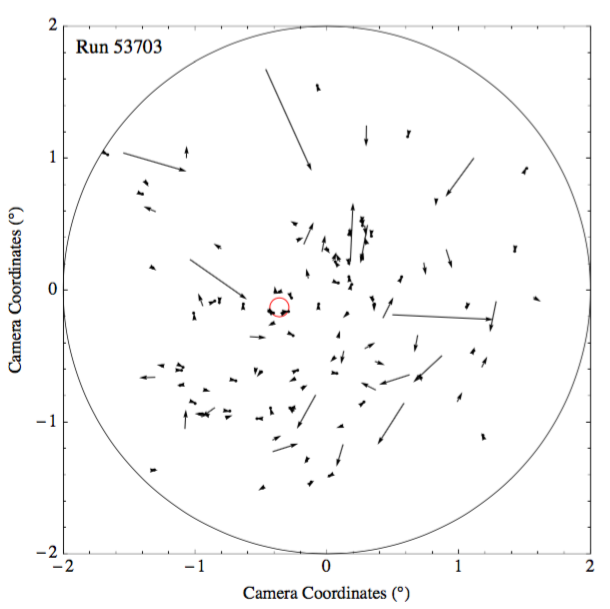
\includegraphics[width=0.8\textwidth]{images/disabled_pixel/moving_events}
      \caption[Event Movement]{
        Positions of events that moved when pixel 115 (denoted by the red circle) was disabled in all four telescopes.  
        Arrows point from the pixel-enabled position to the pixel-disabled position.
      }
      \label{fig:dpix_move}
    \end{figure}

    As the acceptance for a particular event and the event's effective area are strongly related, the loss of acceptance also means a loss of effective area near the pixel.
    This can have effects on the energy reconstruction.
    Additionally, for CTA and its projected \ang{7} diameter field of view, more stars will be in the field of view, implying there will be more camera pixels affected by their light.
    
    {\color{red}(There aren't any bright stars or dead pixels in the Galactic Center data? Tie this back to why this dead pixel study is stil relevant. ??)}
    
    {\color{red}(Again, if I understood correctly that this is negligible, then please preface these two paragraphs by saying that while for VERITAS this effect was found to be negligible, for future experiments like CTA it could be important and then suggest all the ways you think the study can be expanded. Maybe even make it a sub-section in itself. ??)}

    Future studies could also compare how events move in energy when a pixel is disabled.
    Another study might investigate how the reconstructed shower-telescope distance changes, since a shower with fewer pixels will look further away, and may be reconstructed differently.
    In general, as a pixel is disabled, it is expected that lower energy events and showers further away will be more vulnerable, and will show stronger differences than higher energy events or closer showers.


